\documentclass[aspectratio=169, 11pt]{beamer}

\usetheme{metropolis}
\usepackage[sfdefault]{roboto}          
\usepackage[T1]{fontenc}
\usepackage[utf8]{inputenc}
\usepackage{tikz}
\usepackage{pgfplots}
\pgfplotsset{compat=1.18}
\usepgfplotslibrary{groupplots}
\usepackage{booktabs}
\usepackage{appendixnumberbeamer}
\usetikzlibrary{positioning, arrows.meta, fit, backgrounds}

% ---------------------------------------------------------------- colours ---
\definecolor{hsosCyan}{HTML}{009EE3}    
\definecolor{hsosGreen}{HTML}{228B81}   
\definecolor{hsosGreenB}{HTML}{64827D}
\definecolor{hsosGreenC}{HTML}{8CAF90}
\definecolor{hsosOlive}{HTML}{A1AC76}
\definecolor{hsosBlue}{HTML}{678297}
\definecolor{hsosBlueB}{HTML}{85A1B2}
\definecolor{hsosDark}{HTML}{333333}    
\definecolor{hsosGrey}{HTML}{5E5E5D}    
\definecolor{hsosGreyL}{HTML}{CBCCCC}   
\definecolor{hsosPaper}{HTML}{F7F7F7}   

\setbeamercolor{normal text}{fg=hsosDark, bg=white}
\setbeamercolor{alerted text}{fg=hsosGreen}
\setbeamercolor{example text}{fg=hsosCyan}
\setbeamercolor{frametitle}{fg=white, bg=hsosGreen}
\setbeamercolor{title separator}{fg=hsosCyan}
\setbeamercolor{progress bar}{fg=hsosCyan}
\setbeamercolor{palette primary}{fg=white, bg=hsosGreen}
\setbeamercolor{block title}{fg=white, bg=hsosGreen}
\setbeamercolor{block body}{bg=hsosPaper}
\setbeamercolor{footline}{fg=hsosGrey}

\metroset{numbering=fraction, progressbar=frametitle, block=fill}
\setbeamertemplate{navigation symbols}{}
\setbeamertemplate{frametitle continuation}{}   
\setbeamertemplate{bibliography item}[text]     

\newcommand{\srcnote}[1]{%
  \begin{tikzpicture}[remember picture, overlay]
    \node[anchor=south west, text=hsosGrey, font=\tiny,
          xshift=0.9cm, yshift=0.45cm] at (current page.south west) {#1};
  \end{tikzpicture}}

\newcommand{\stat}[3]{%
  \begin{minipage}[t]{#1}\centering
    {\Large\color{hsosGreen}#2}\\[0.15em]
    {\footnotesize\color{hsosGrey}#3}
  \end{minipage}}

% ------------------------------------------------------------ bibliography ---
\usepackage[backend=biber, style=numeric, sorting=none, maxcitenames=2, maxbibnames=3,
            giveninits=true, doi=false, isbn=false, url=false, eprint=false]{biblatex}
\addbibresource{../paper/bibliography.bib}
\renewcommand*{\bibfont}{\scriptsize}

\title{Mind the Gap}
\subtitle{Joint vs.\ Data-Incremental Self-Supervised Pretraining\\for Plant
Classification}
\author{\textbf{Andreas Schliebitz} \and Heiko Tapken \and Martin Atzmueller}
% Everything after the authors goes in \institute so the affiliations precede
% the venue; metropolis would otherwise print the date between them.
\institute{%
  \footnotesize Osnabrück University of Applied Sciences\\
  \footnotesize Osnabrück University, Semantic Information Systems Group\\[0.8em]
  \footnotesize\color{hsosGrey}GIL-Jahrestagung 2027 · Souveränität in der
  Land-, Forst- und Ernährungswirtschaft\\
  \footnotesize\color{hsosGrey}Lecture Notes in Informatics (LNI) ·
  Gesellschaft für Informatik · Triesdorf 2027}
\date{}

\begin{document}

\maketitle

% =============================================================== motivation ==
\begin{frame}{Agricultural image collections are never finished}
  \centering
  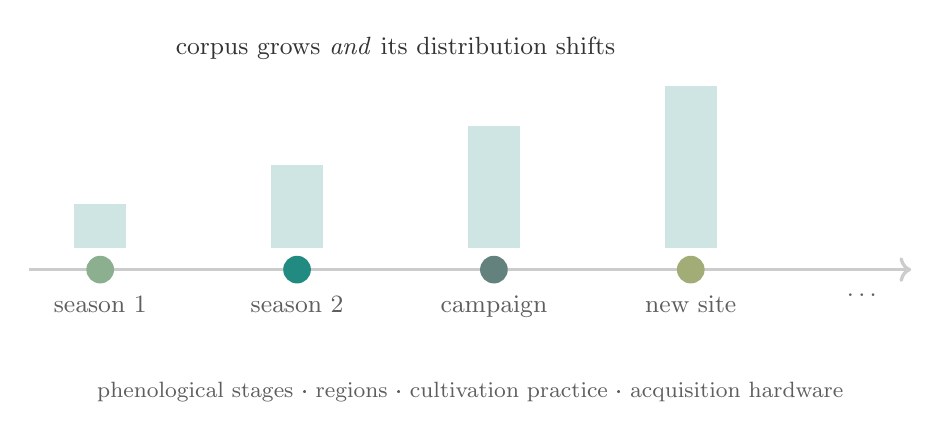
\begin{tikzpicture}[font=\small]
    \draw[->, very thick, hsosGreyL] (0,0) -- (11.2,0);
    \foreach \x/\lab/\col in {0.9/season 1/hsosGreenC, 3.4/season 2/hsosGreen,
                              5.9/campaign/hsosGreenB, 8.4/new site/hsosOlive} {
      \fill[\col] (\x,0) circle (5pt);
      \node[below=6pt, text=hsosGrey] at (\x,0) {\lab};
    }
    \node[text=hsosGrey] at (10.6,-0.33) {\dots};
    \foreach \x/\h in {0.9/0.55, 3.4/1.05, 5.9/1.55, 8.4/2.05} {
      \fill[hsosGreen!22] (\x-0.33,0.28) rectangle (\x+0.33,\h+0.28);
    }
    \node[above, text=hsosDark] at (4.65,2.55)
      {\small corpus grows \emph{and} its distribution shifts};
    \node[below=1.3cm, text=hsosGrey, align=center, font=\footnotesize] at (5.6,0)
      {phenological stages · regions · cultivation practice · acquisition hardware};
  \end{tikzpicture}

  \vspace{0.7em}
  {\color{hsosGrey}Every arrival poses the same question: what do we do with the encoder?}
  \srcnote{Deep learning as the default tool for such imagery: \textcite{Kamilaris2018}}
\end{frame}

% ================================================================= decision ==
\begin{frame}{Two ways to absorb new data}
  \centering
  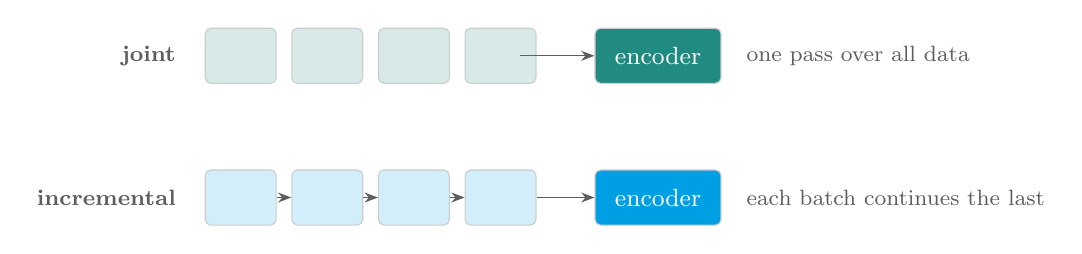
\begin{tikzpicture}[font=\small, node distance=4mm,
      box/.style={rounded corners=2pt, draw=hsosGreyL, fill=hsosPaper,
                  minimum height=7mm, minimum width=9mm, inner sep=2pt},
      lbl/.style={text=hsosGrey, font=\footnotesize}]
    % joint
    \node[lbl, anchor=east] at (-0.7,1.5) {\textbf{joint}};
    \foreach \i in {0,1,2,3} \node[box, fill=hsosGreen!18] (j\i) at (\i*1.1,1.5) {};
    \node[box, fill=hsosGreen, text=white, minimum width=16mm] (jm) at (5.3,1.5) {encoder};
    \draw[-{Stealth}, hsosGrey] (3.55,1.5) -- (jm.west);
    \node[lbl, anchor=west] at (6.3,1.5) {one pass over all data};
    % incremental
    \node[lbl, anchor=east] at (-0.7,-0.3) {\textbf{incremental}};
    \foreach \i in {0,1,2,3} {
      \node[box, fill=hsosCyan!18] (c\i) at (\i*1.1,-0.3) {};
    }
    \foreach \i/\j in {0/1,1/2,2/3} \draw[-{Stealth}, hsosGrey] (c\i) -- (c\j);
    \node[box, fill=hsosCyan, text=white, minimum width=16mm] (cm) at (5.3,-0.3) {encoder};
    \draw[-{Stealth}, hsosGrey] (c3) -- (cm.west);
    \node[lbl, anchor=west] at (6.3,-0.3) {each batch continues the last};
  \end{tikzpicture}

  \vspace{1.2em}
  {\color{hsosGrey}Incremental is cheaper and does not presuppose that earlier
  images are still available.}\\[0.3em]
  {\color{hsosDark}\textbf{What does it cost in representation quality?}}
\end{frame}

% ======================================================== labelling costs ====
\begin{frame}{Labels are not equally expensive}
  \centering
  \vspace{0.3em}
  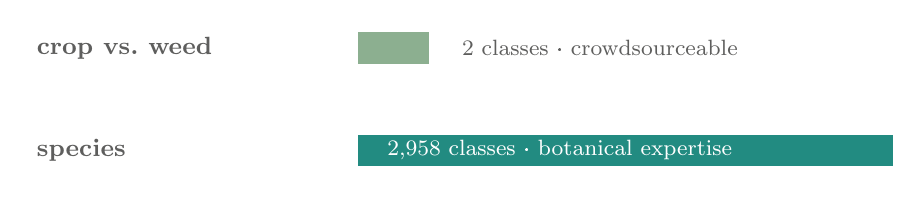
\begin{tikzpicture}[font=\small]
    \node[text=hsosGrey, anchor=west] at (0,2.3) {\textbf{crop vs.\ weed}};
    \fill[hsosGreenC] (4.2,2.1) rectangle (5.1,2.5);
    \node[anchor=west, text=hsosGrey, font=\footnotesize] at (5.4,2.3)
      {2 classes · crowdsourceable};

    \node[text=hsosGrey, anchor=west] at (0,1.0) {\textbf{species}};
    \fill[hsosGreen] (4.2,0.8) rectangle (11.0,1.2);
    \node[anchor=west, text=white, font=\footnotesize] at (4.45,1.0)
      {2{,}958 classes · botanical expertise};
  \end{tikzpicture}

  \vspace{1.0em}
  \begin{columns}[T]
    \column{0.82\textwidth}
    \centering
    {\color{hsosDark}Self-supervised pretraining decouples the two: train the
    encoder on \textbf{unlabelled} images, freeze it,\\ then fit a small probe for
    whichever target you can afford to label.}
  \end{columns}
  \srcnote{\textcite{VanHorn2018}; \textcite{Jain2025}; SSL on agricultural
           imagery: \textcite{Gueldenring2021}}
\end{frame}

% ================================================================= question ==
{\setbeamercolor{palette primary}{fg=hsosGreyL, bg=hsosGreen}
 \setbeamercolor{alerted text}{fg=white}
 \setbeamercolor{footline}{fg=hsosGreyL}
\begin{frame}[standout]
  Does the cost of pretraining \emph{incrementally}\\[0.3em]
  depend on the \alert{granularity} of the labels\\[0.3em]
  you later evaluate on?
\end{frame}}

% ===================================================================== data ==
\begin{frame}{One encoder, four nested targets}
  \centering
  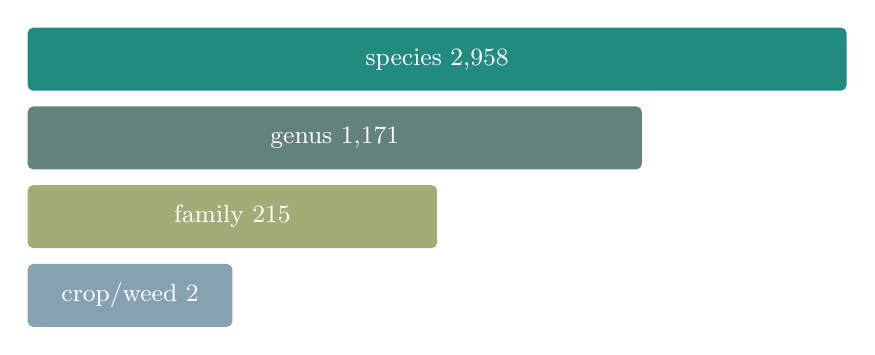
\begin{tikzpicture}[font=\small,
      lvl/.style={rounded corners=2pt, text=white, minimum height=8mm,
                  inner xsep=6pt, font=\small}]
    \node[lvl, fill=hsosGreen,  minimum width=10.4cm] (s) at (0,2.1) {species \hfill 2{,}958};
    \node[lvl, fill=hsosGreenB, minimum width=7.8cm]  (g) at (-1.3,1.1) {genus \hfill 1{,}171};
    \node[lvl, fill=hsosOlive,  minimum width=5.2cm]  (f) at (-2.6,0.1) {family \hfill 215};
    \node[lvl, fill=hsosBlueB,  minimum width=2.6cm]  (c) at (-3.9,-0.9) {crop/weed \hfill 2};
  \end{tikzpicture}

  \vspace{1.0em}
  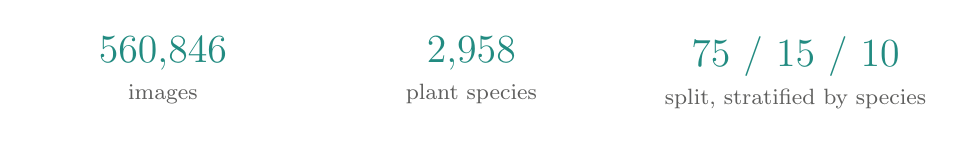
\begin{tikzpicture}
    \node {\stat{3.2cm}{560{,}846}{images}\hspace{0.6cm}
           \stat{3.2cm}{2{,}958}{plant species}\hspace{0.6cm}
           \stat{3.6cm}{75 / 15 / 10}{split, stratified by species}};
  \end{tikzpicture}

  \vspace{0.3em}
  {\color{hsosGrey}\footnotesize The hierarchy is strictly nested, so a single
  frozen encoder serves all four probes.}
  \srcnote{iNatAg-mini: \textcite{Jain2025}; taxonomy metadata: \textcite{Joshi2023}}
\end{frame}

% =================================================== compute-matched design ==
\begin{frame}{A fair comparison: identical compute}
  \centering
  \vspace{0.2em}
  \begin{tikzpicture}[font=\small,
      seg/.style={rounded corners=1pt, draw=none, minimum height=6mm}]
    \node[text=hsosGrey, anchor=east, font=\footnotesize] at (-0.2,1.6) {joint};
    \node[seg, fill=hsosGreen, text=white, minimum width=8.8cm] at (4.4,1.6)
      {100 epochs over the full training split};

    \node[text=hsosGrey, anchor=east, font=\footnotesize] at (-0.2,0.4) {$N=2$};
    \foreach \i in {0,1} \node[seg, fill=hsosCyan!70, text=white,
      minimum width=4.3cm] at (\i*4.5+2.15,0.4) {100 epochs · \(\tfrac12\) data};

    \node[text=hsosGrey, anchor=east, font=\footnotesize] at (-0.2,-0.8) {$N=8$};
    \foreach \i in {0,...,7} \node[seg, fill=hsosCyan!45,
      minimum width=1.0cm] at (\i*1.1+0.55,-0.8) {};
  \end{tikzpicture}

  \vspace{1.1em}
  
\begin{tikzpicture}
    \node {\stat{4.0cm}{219{,}000}{optimizer steps, both arms}\hspace{0.8cm}
           \stat{4.0cm}{100$\times$}{every image seen, both arms}};
  \end{tikzpicture}

  \vspace{0.5em}
  {\color{hsosGrey}\small Only the \emph{order} in which the data arrives differs.
  DINOv2 ViT-S/14, trained from random initialization.}
  \srcnote{DINOv2: \textcite{Oquab2024}; instance-incremental streams:
           \textcite{Douillard2021}}
\end{frame}

% ============================================================ stream orders ==
\begin{frame}{Two ways to cut the stream}
  \vspace{0.3em}
  \begin{columns}[T, onlytextwidth]
    \column{0.47\textwidth}
      \textbf{\color{hsosGreen}i.i.d.}\\[0.4em]
      {\color{hsosGrey}Every segment contains all 2{,}958 species.\\
      Isolates the effect of \emph{sequential presentation} alone.}\\[0.6em]
      \stat{\textwidth}{100\,\% coverage}{in every segment}
    \column{0.47\textwidth}
      \textbf{\color{hsosCyan}seasonal}\\[0.4em]
      {\color{hsosGrey}Ordered by month of capture, hemisphere corrected.\\
      Deliberately introduces \emph{covariate shift}.}\\[0.6em]
      \stat{\textwidth}{87.4--94.0\,\%}{species coverage at $N=8$}
  \end{columns}
  \vspace{1.0em}
  \centering
  {\color{hsosGrey}\small Ordering by absolute date was measured and rejected:
  50.9\,\% of the corpus falls in a single year.}
\end{frame}

% =============================================================== evaluation ==
\begin{frame}{Evaluation: freeze, then probe}
  \centering
  \vspace{0.6em}
  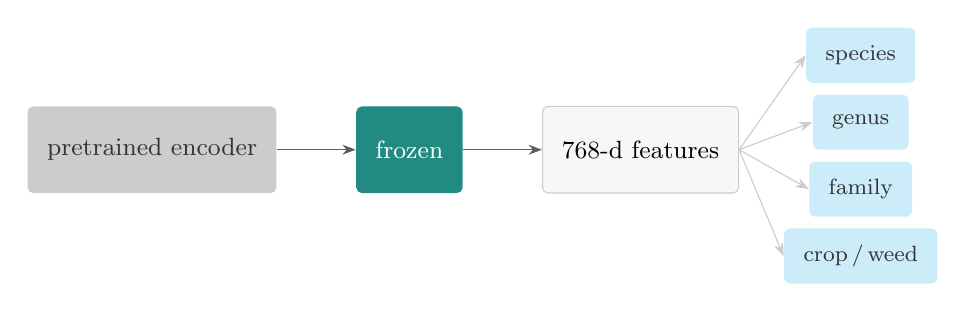
\begin{tikzpicture}[font=\small, node distance=8mm,
      b/.style={rounded corners=2pt, minimum height=11mm, inner xsep=7pt}]
    \node[b, fill=hsosGreyL, text=hsosDark] (enc) {pretrained encoder};
    \node[b, fill=hsosGreen, text=white, right=10mm of enc] (frz) {frozen};
    \node[b, fill=hsosPaper, draw=hsosGreyL, right=10mm of frz] (feat) {768-d features};
    \draw[-{Stealth}, hsosGrey] (enc) -- (frz);
    \draw[-{Stealth}, hsosGrey] (frz) -- (feat);
    \foreach \i/\n in {0/species, 1/genus, 2/family, 3/{crop\,/\,weed}} {
      \node[b, fill=hsosCyan!20, text=hsosDark, font=\footnotesize,
            minimum height=7mm] (p\i) at (9.0, 1.2-\i*0.85) {\n};
      \draw[-{Stealth}, hsosGreyL] (feat.east) -- (p\i.west);
    }
  \end{tikzpicture}

  \vspace{1.0em}
  {\color{hsosGrey}\small Linear probes only. The encoder is never fine-tuned,
  so every difference comes from the representation itself.}\\[0.3em]
  {\color{hsosGrey}\small Reported as micro-averaged top-1 accuracy.}
\end{frame}

% ============================================================ headline result ==
\begin{frame}{The penalty depends on granularity}
  \centering
  \vspace{-0.2em}
  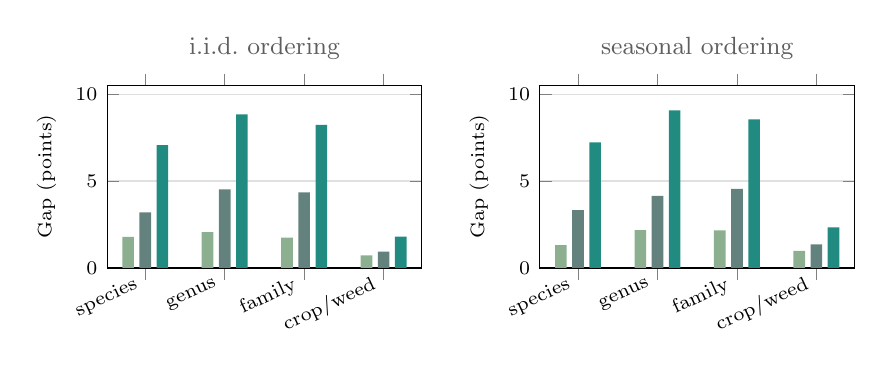
\begin{tikzpicture}
    \begin{groupplot}[
      group style={group size=2 by 1, horizontal sep=1.5cm},
      width=0.46\linewidth, height=3.9cm,
      ybar, /pgf/bar width=4.2pt,
      symbolic x coords={species,genus,family,crop/weed},
      xtick=data, x tick label style={font=\scriptsize, rotate=25, anchor=east},
      y tick label style={font=\scriptsize},
      ymin=0, ymax=10.5, ylabel={Gap (points)}, ylabel style={font=\scriptsize},
      enlarge x limits=0.16, ymajorgrids=true, grid style={hsosGreyL!60},
      title style={font=\small, text=hsosGrey},
      legend style={legend columns=3, draw=none, fill=none, font=\scriptsize},
      every axis plot/.append style={draw=none},
    ]
    \nextgroupplot[title={i.i.d.\ ordering}, legend to name=gaplegend]
    \addplot[fill=hsosGreenC] coordinates {(species,1.79) (genus,2.06) (family,1.74) (crop/weed,0.73)};
    \addplot[fill=hsosGreenB] coordinates {(species,3.20) (genus,4.52) (family,4.35) (crop/weed,0.94)};
    \addplot[fill=hsosGreen]  coordinates {(species,7.06) (genus,8.84) (family,8.23) (crop/weed,1.81)};
    \legend{$N=2$,$N=4$,$N=8$}
    \nextgroupplot[title={seasonal ordering}]
    \addplot[fill=hsosGreenC] coordinates {(species,1.32) (genus,2.17) (family,2.16) (crop/weed,0.99)};
    \addplot[fill=hsosGreenB] coordinates {(species,3.33) (genus,4.15) (family,4.55) (crop/weed,1.35)};
    \addplot[fill=hsosGreen]  coordinates {(species,7.22) (genus,9.06) (family,8.55) (crop/weed,2.33)};
    \end{groupplot}
  \end{tikzpicture}\\[0.2em]
  \ref{gaplegend}

  \vspace{0.4em}
  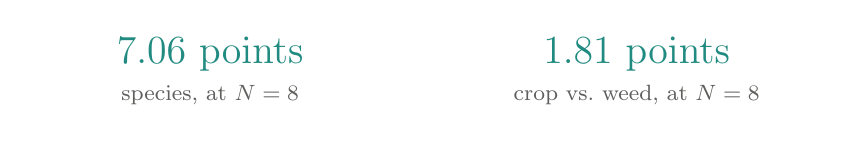
\begin{tikzpicture}
    \node {\stat{4.4cm}{7.06 points}{species, at $N=8$}\hspace{0.9cm}
           \stat{4.4cm}{1.81 points}{crop vs.\ weed, at $N=8$}};
  \end{tikzpicture}
\end{frame}

% ============================================================ relative view ==
\begin{frame}{Eight times the damage, same encoder}
  \centering
  \vspace{0.9em}
  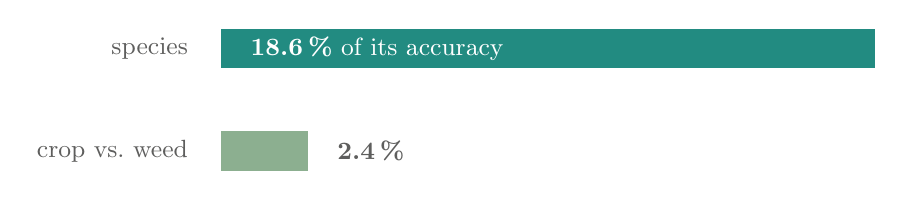
\begin{tikzpicture}[font=\small]
    \node[text=hsosGrey, anchor=east] at (0,1.6) {species};
    \fill[hsosGreen] (0.3,1.35) rectangle (8.6,1.85);
    \node[anchor=west, text=white] at (0.55,1.6) {\textbf{18.6\,\%} of its accuracy};

    \node[text=hsosGrey, anchor=east] at (0,0.3) {crop vs.\ weed};
    \fill[hsosGreenC] (0.3,0.05) rectangle (1.4,0.55);
    \node[anchor=west, text=hsosGrey] at (1.65,0.3) {\textbf{2.4\,\%}};
  \end{tikzpicture}

  \vspace{1.4em}
  {\color{hsosDark}Relative to the jointly trained baseline, at eight segments.}\\[0.5em]
  {\color{hsosGrey}The gap grows monotonically with segment count, and the two
  orderings agree closely.}
\end{frame}

% =============================================================== trajectory ==
\begin{frame}{Most of the deficit is recovered, but not all}
  \centering
  \vspace{-0.1em}
  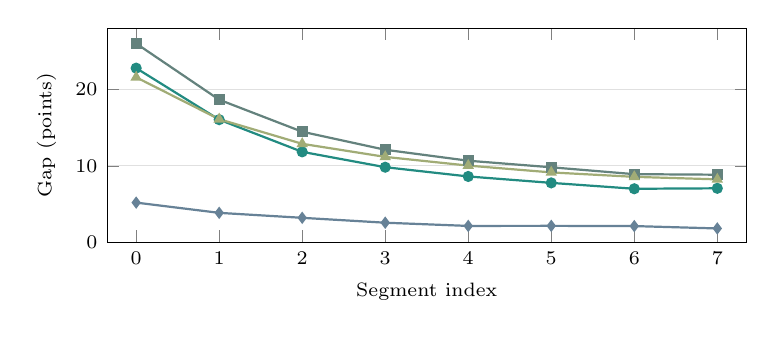
\begin{tikzpicture}
    \begin{axis}[
      width=0.80\linewidth, height=4.3cm,
      xlabel={Segment index}, ylabel={Gap (points)},
      label style={font=\scriptsize}, tick label style={font=\scriptsize},
      xmin=-0.35, xmax=7.35, ymin=0, ymax=28, xtick={0,...,7},
      ymajorgrids=true, grid style={hsosGreyL!60},
      legend to name=trajlegend,
      legend style={legend columns=4, draw=none, fill=none, font=\scriptsize},
      mark size=1.6pt, every axis plot/.append style={thick},
    ]
    \addplot[hsosGreen, mark=*]        coordinates {(0,22.78)(1,16.04)(2,11.83)(3,9.82)(4,8.61)(5,7.77)(6,7.00)(7,7.06)};
    \addplot[hsosGreenB, mark=square*] coordinates {(0,26.00)(1,18.65)(2,14.46)(3,12.10)(4,10.67)(5,9.81)(6,8.91)(7,8.84)};
    \addplot[hsosOlive, mark=triangle*] coordinates {(0,21.58)(1,16.10)(2,12.88)(3,11.17)(4,10.03)(5,9.14)(6,8.56)(7,8.23)};
    \addplot[hsosBlue, mark=diamond*]  coordinates {(0,5.19)(1,3.85)(2,3.20)(3,2.56)(4,2.14)(5,2.15)(6,2.12)(7,1.81)};
    \legend{species,genus,family,crop/weed}
    \end{axis}
  \end{tikzpicture}\\[0.1em]
  \ref{trajlegend}

  \vspace{0.5em}
  {\color{hsosGrey}\small The large initial deficit reflects limited data, not
  forgetting. The residual is what the previous slide quantifies.}
\end{frame}

% ================================================================ mechanism ==
\begin{frame}{The representation drifts}
  \vspace{0.8em}
  \centering
  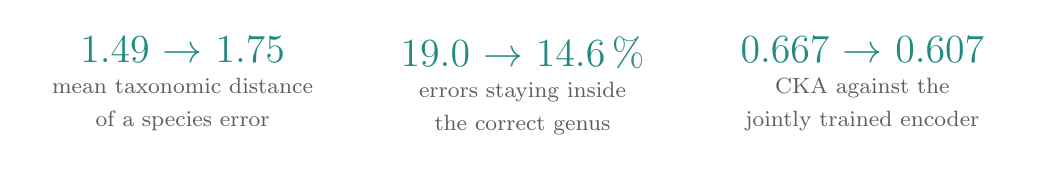
\begin{tikzpicture}
    \node {\stat{3.7cm}{1.49 $\rightarrow$ 1.75}{mean taxonomic distance\\of a species error}\hspace{0.5cm}
           \stat{3.7cm}{19.0 $\rightarrow$ 14.6\,\%}{errors staying inside\\the correct genus}\hspace{0.5cm}
           \stat{3.7cm}{0.667 $\rightarrow$ 0.607}{CKA against the\\jointly trained encoder}};
  \end{tikzpicture}

  \vspace{1.6em}
  {\color{hsosDark}All three move monotonically with segment count, and all three
  point the same way.}\\[0.4em]
  {\color{hsosGrey}Errors do not merely become more frequent, they land further
  from the truth in the taxonomy.}
  \srcnote{Centred kernel alignment: \textcite{Kornblith2019}}
\end{frame}

% ============================================================== fragmenting ==
\begin{frame}{Fragmentation, not distribution shift}
  \vspace{1.1em}
  \centering
  
\begin{tikzpicture}[font=\small]
    \node[text=hsosGrey, anchor=east] at (0,1.2) {i.i.d.\ (full coverage)};
    \fill[hsosGreen] (0.3,0.95) rectangle (7.36,1.45);
    \node[anchor=west, text=white] at (0.55,1.2) {\textbf{7.06} points at species};

    \node[text=hsosGrey, anchor=east] at (0,0.1) {seasonal (shifted)};
    \fill[hsosCyan] (0.3,-0.15) rectangle (7.52,0.35);
    \node[anchor=west, text=white] at (0.55,0.1) {\textbf{7.22} points at species};
  \end{tikzpicture}

  \vspace{1.5em}
  {\color{hsosDark}Breaking coverage barely changes the outcome.}\\[0.4em]
  {\color{hsosGrey}Within the range of shift this corpus admits, the penalty is
  driven by \emph{how often the stream is cut}, not by what is in each piece.}
\end{frame}

% ================================================================= takeaways ==
\begin{frame}{What this means in practice}
  \vspace{0.9em}
  \begin{columns}[T, onlytextwidth]
    \column{0.31\textwidth}
      {\color{hsosGreen}\large\textbf{1}}\\[0.4em]
      {\color{hsosDark}Coarse tasks tolerate incremental updates.}\\[0.3em]
      {\color{hsosGrey}\footnotesize Crop vs.\ weed loses 1.81 points, exactly
      where labels are cheap and updates frequent.}
    \column{0.31\textwidth}
      {\color{hsosGreen}\large\textbf{2}}\\[0.4em]
      {\color{hsosDark}Fine-grained targets do not.}\\[0.3em]
      {\color{hsosGrey}\footnotesize Species forfeits close to a fifth of its
      accuracy, and further segments do not recover it.}
    \column{0.31\textwidth}
      {\color{hsosGreen}\large\textbf{3}}\\[0.4em]
      {\color{hsosDark}One aggregate score hides this.}\\[0.3em]
      {\color{hsosGrey}\footnotesize Averaging the four levels reports about six
      points and conceals both ends.}
  \end{columns}

  \vspace{1.5em}
  \centering
  {\color{hsosGrey}\small Where one frozen encoder serves both, the finest
  downstream target dictates the update strategy.}
  \srcnote{Aggregate reporting is the norm in continual SSL:
           \textcite{Fini2022}; \textcite{Purushwalkam2022}; \textcite{Madaan2022}}
\end{frame}

% ====================================================== limits / future work ==
\begin{frame}{Limitations and what comes next}
  \vspace{0.7em}
  \begin{columns}[T, onlytextwidth]
    \column{0.46\textwidth}
      {\color{hsosGrey}\textbf{Bounds on these conclusions}}\\[0.5em]
      {\footnotesize
      \color{hsosDark}Single seed per configuration; the claim rests on the
      monotone trend replicated under two orderings.\\[0.4em]
      The schedule restarts at every boundary, so the measured gap is an
      \emph{upper bound} on the ordering effect.\\[0.4em]
      560k images, one architecture, one objective.}
    \column{0.46\textwidth}
      {\color{hsosGreen}\textbf{Next steps}}\\[0.5em]
      {\footnotesize
      \color{hsosDark}How small a replay buffer closes the species gap, and does
      that budget itself depend on granularity?\\[0.4em]
      Does distillation preserve fine structure, or only lift the aggregate?\\[0.4em]
      Hierarchy-aware objectives, and the full 4.7M-image release.}
  \end{columns}
  \srcnote{Distillation for continual SSL: \textcite{Fini2022};
           full release: \textcite{Jain2025}}
\end{frame}

% =============================================================== references ==
\begin{frame}[allowframebreaks]{References}
  \printbibliography[heading=none]
\end{frame}

% =================================================================== thanks ==
{\setbeamercolor{footline}{fg=hsosGreyL}
\begin{frame}[standout]
  Thank you for your attention.

  \vspace{0.7em}
  {\normalsize\color{white}Questions?}

  \vspace{1.5em}
  {\footnotesize\color{hsosGreyL}a.schliebitz@hs-osnabrueck.de}
\end{frame}}

\end{document}
